%%%%%%%%%%%%%%%%%%%%%%%%%%%%%%%%%%%%%%%%%
% Journal Article
% LaTeX Template
% Version 1.4 (15/5/16)
%
% This template has been downloaded from:
% http://www.LaTeXTemplates.com
%
% Original author:
% Frits Wenneker (http://www.howtotex.com) with extensive modifications by
% Vel (vel@LaTeXTemplates.com)
%
% License:
% CC BY-NC-SA 3.0 (http://creativecommons.org/licenses/by-nc-sa/3.0/)
%
%%%%%%%%%%%%%%%%%%%%%%%%%%%%%%%%%%%%%%%%%

%----------------------------------------------------------------------------------------
%	PACKAGES AND OTHER DOCUMENT CONFIGURATIONS
%----------------------------------------------------------------------------------------

\documentclass[twoside,twocolumn]{article}
\usepackage[utf8]{inputenc}
\usepackage{blindtext} % Package to generate dummy text throughout this template 
\usepackage{dblfloatfix}
\usepackage[sc]{mathpazo} % Use the Palatino font
\usepackage[T1]{fontenc} % Use 8-bit encoding that has 256 glyphs
\linespread{1.05} % Line spacing - Palatino needs more space between lines
\usepackage{microtype} % Slightly tweak font spacing for aesthetics
\usepackage{graphicx}
\usepackage[french]{babel} % Language hyphenation and typographical rules

\usepackage[hmargin=2cm,vmargin=2.5cm,bindingoffset=0cm]{geometry}
\usepackage[hang, small,labelfont=bf,up,textfont=it,up]{caption} % Custom captions under/above floats in tables or figures
\usepackage{booktabs} % Horizontal rules in tables

\usepackage{lettrine} % The lettrine is the first enlarged letter at the beginning of the text

\usepackage{enumitem} % Customized lists
\setlist[itemize]{noitemsep} % Make itemize lists more compact

\usepackage{abstract} % Allows abstract customization
\renewcommand{\abstractnamefont}{\normalfont\bfseries} % Set the "Abstract" text to bold
\renewcommand{\abstracttextfont}{\normalfont\small\itshape} % Set the abstract itself to small italic text

\usepackage{titlesec} % Allows customization of titles
\renewcommand\thesection{\Roman{section}} % Roman numerals for the sections
\renewcommand\thesubsection{\arabic{subsection}} % roman numerals for subsections
\titleformat{\section}[block]{\large\scshape\centering}{\thesection.}{1em}{} % Change the look of the section titles
\titleformat{\subsection}[block]{\bfseries\large}{\thesubsection.}{1em}{} % Change the look of the section titles

\usepackage{fancyhdr} % Headers and footers
\pagestyle{fancy} % All pages have headers and footers
\fancyhead{} % Blank out the default header
\fancyfoot{} % Blank out the default footer
\fancyhead[C]{Manifold learning$\bullet$Nogueira, Tevi, Keleko $\bullet$ Decembre 2016} % Custom header text
\fancyfoot[RO,LE]{\thepage} % Custom footer text

\usepackage{titling} % Customizing the title section

\usepackage[hidelinks=true]{hyperref} % For hyperlinks in the PDF
\usepackage{xcolor}
\hypersetup{colorlinks,linkcolor={red!50!black}, citecolor={blue!50!black}, urlcolor={blue!80!black}}
%\hypersetup{frenchlinks=true}
\usepackage{amsmath}

%\usepackage{placeins}
%\let\Oldsection\section
%\renewcommand{\section}{\FloatBarrier\Oldsection}

%----------------------------------------------------------------------------------------
%	TITLE SECTION
%----------------------------------------------------------------------------------------

\setlength{\droptitle}{-4\baselineskip} % Move the title up

\pretitle{\begin{center}\Huge\bfseries} % Article title formatting
\posttitle{\end{center}} % Article title closing formatting
\title{ETUDE COMPARATIVE DES METHODES DE REDUCTION
DE LA DIMENSION 
} % Article title
\author{%
\textsc{Iuri D. Nogueira, Lauriane Tele Tevi, Aurelien Keleko T.} \\[1ex] % Your name
\normalsize Université Lumiere Lyon 2 \\ % Your institution
\normalsize Master 2 Data Mining  
%\normalsize \href{mailto:john@smith.com}{john@smith.com} % Your email address
%\and % Uncomment if 2 authors are required, duplicate these 4 lines if more
%\textsc{Jane Smith}\thanks{Corresponding author} \\[1ex] % Second author's name
%\normalsize University of Utah \\ % Second author's institution
%\normalsize \href{mailto:jane@smith.com}{jane@smith.com} % Second author's email address
}
%\date{\today} % Leave empty to omit a date
\renewcommand{\maketitlehookd}{%
\begin{abstract}
\noindent Durant ses dernières décennies nous avons assistés au développement de plusieurs techniques non-linéaires pour la réduction de la dimension. Celles-ci ont souvent démontrées certaines limites et défaillances par rapport aux techniques linéaires classiques telles que l’analyse en composantes principales.
Cet article met en évidence les principales différences qui existent entre les méthodes linéaires et non-linéaires. Ces techniques seront appliquées sur des jeux de données et proposeront des suggestions et des résultats. Toutefois ses résultats mettront en exergue la fragilité de certaines techniques non linéaires, qui sont sensibles aux phénomènes de bruit, de grande dimension, et peuvent donc être améliorées.


\medskip
\textbf{Mots clés} 
Réduction de la dimension, manifold, PCA, LLE, ISOMAP, MDS, Sammon, métrique, dimension intrinsèque, distance euclidienne, indice de similarité, projection et méthode linéaire.  
\end{abstract}
}
%----------------------------------------------------------------------------------------

\begin{document}

% Print the title
\maketitle

%----------------------------------------------------------------------------------------
%	ARTICLE CONTENTS
%----------------------------------------------------------------------------------------

\section{Introduction et objectifs}

\lettrine[nindent=0em,lines=2]{G} 
enéralement les données proviennent de sources diverses et hétérogènes par exemple les capteurs, les radiographies, les smartphones et les antennes. Elles sont de grande dimension et peuvent être de différentes formes: images, sons, ondes, numériques et graphes.
Pour la fiabilité des analyses il est indispensable de réduire la dimension des données, générant des redondances qui engendrent des incohérences statistiques et altèrent la connaissance des données.  
L’objectif principal de ces techniques consiste à sélectionner un sous ensemble optimal dont la taille intrinsèque qui représente les données sans trop déformer la réalité de la dimension extrinsèque. Ainsi cette réduction confère plusieurs avantages tels le gain de mémoire, la réduction du temps d’exécution, la facilité des traitements, d'analyse, et d'interprétations : clustering, classification et visualisation des données en grande dimension. En somme elle aide à comprendre le phénomène étudié.
Il existe plusieurs approches pour réduire la redondance dans les données, la technique de réduction linéaire de la dimension dans ce cas est l’analyse de composantes principales (PCA). Cependant l’efficacité de cette méthode a été démontrée car elle ne permet pas de gérer les données fonctionnelles et non linéaires. Pour palier à ce défaut, il a été développé d’autres approches qui sont plus performantes lorsque les données sont complexes ce qui est le cas dans le monde réel. Les techniques non linéaires fonctionnent bien avec des données simulées mais pas toujours avec des données naturelles. Nous ne pouvons donc pas affirmer l’existence d’une stratégie absolue pour réduire de manière significative la dimension des données.

Cet article présente une étude comparative sur les méthodes de réduction de la dimension, du point de vue empirique, théorique et computationnel. Premièrement nous présenterons une technique linéaire: PCA, ensuite nous illustrerons trois méthodes non linéaires: l’Isometric Feature Mapping, Locally Linear Embedding et Sammon Mapping. Puis nous présenterons les objectifs, les détails des choix techniques et la description des données simulées. La troisième partie traitera de l’application de ses techniques sur des données artificielles et réelles. Enfin nous présenterons les différentes comparaisons, performances et résultats obtenus.



%------------------------------------------------

\section{Principe de réduction de la dimension}

Soit $\mathbf{X}$ une matrice de données de dimension n x D,
$\mathbf{X}=X_1,X_2, ... ,X_n$. On suppose que la vraie dimension de ce vecteur est $\mathbf Y$ tel que: $\mathbf{Y}=Y_1,Y_2, ..., Y_n$ de dimension $n x d$.

\begin{itemize}
\item $\mathbf D$: dimension extrinsèque.
\item $\mathbf d$: dimension intrinsèque.
\end{itemize}

L’objectif principal de ses techniques est d’avoir un jeu de données de dimension réduite tel que $ d < <  D$ qui minimise la perte d’information et en ayant aucune hypothèse sur la structure des données (Fig. \ref{prinp}). 
\begin{figure}[ht!]
  \centering
  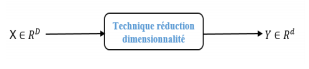
\includegraphics[width= \linewidth]{01.png} 
  \vspace{-24pt}
  \caption{Principe de réduction de la dimension}
  \label{prinp}
\end{figure}

\section{Description des techniques de réduction de la dimension}

Les techniques de réduction de la dimension sont multiples,il existe deux grandes familles: convexe et non convexe. Parmi les méthodes convexes on retrouve celles entièrement spectrales basées sur la notion de distance: PCA (linéaire), ISOMAP (non-linéaire) et celles partiellement spectrales basées sur la notion de structure: LLE (non linéaire). Pour les techniques non convexes on a celles basées sur le poids de la distance euclidienne: Sammon Mapping (non linéaire).

\begin{enumerate}
\item PCA: Principal Component Analysis
\item ISOMAP: Isometric Feature Mapping
\item LLE: Locally Linear Embedding
\item Sammon Mapping
\end{enumerate}


\subsection{Technique linéaire: Analyse de Composante Principale (PCA)}
 
L’analyse des composantes principales (PCA) a été introduite par Karl Pearson en 1901, il s’agit de l’une des techniques traditionnelles linéaires qui permet la réduction de la dimension. Son principe est de maximiser la variance sur les données projetées en minimisant au plus les déformations de ses projections. Elle offre la possibilité de réduire voir d'éliminer la redondance dans les données corrélées. Par contre elle ne garde pas toutes les informations complémentaires pendant la projection et ne préserve pas la complexité de ses structures. En somme elle permet d’avoir un ensemble de données initiales qui est représenté par un autre ensemble réduit de variable.\cite{Wang12}

La PCA peut être décrite sur plusieurs points de vue: statistiques et géométriques.Secondement elle consiste à faire une projection linéaire sur le sous-espace engendré par les $p$vecteurs propres de la matrice de covariance en maximisant l’inertie entre ceux-ci. Pour cette étude nous aborderons l’aspect statistique et utiliserons les notions de distance euclidienne et de similarité entre les variables.  
Soit l’ensemble des données d’origine:
$ \mathbf{X \subset R^D}$ et l’ensemble des données d’arrivées réduites $\mathbf{Y \subset R^d}$. En considérant la  distance euclidienne on cherche une projection linéaire $\mathbf{ F: R^D \rightarrow R^d}$ tel que : $\mathbf{Y = F(X)}$ qui  maximise l’inertie entre les données. \cite{Wang12} 

Soit $\mathbf {x} =[x_1, x_2, ..., x_n]$ une matrice représentative de $\mathbb{ X \subset R^D}$, chaque colonne de $\mathbf{x_i \in X}$ est considéré comme une observation du vecteur. Pour des raisons techniques nous allons normaliser le vecteur aléatoire $\mathbb{X}$. 
\begin{itemize}
\item Centrer le vecteur $\mathbb{X_i}$

$\mathbf{E(X_i)}=\mu=0$ pour $ \forall$ $\mathbf{i}=1, 2, .., n$
\item Calculer la variance du vecteur $\mathbb{X_i}$ \\
$\mathbf{Var(X_i)}=\frac{1}{n}\sum_{i=1}^{n}( x_i-\mu )^2$ sachant que $\mu=0$
on obtient une forme plus simplifiée de la variance $\mathbb{X_i}$ 
$\mathbf{Var(X_i)}=\frac{1}{n}\sum_{i=1}^{n}\left(x_i\right)^2$
\end{itemize}

Soit $v_1$ la première direction principal du vecteur aléatoire $X$ de dimension $D$ tel que $ \mathbf{v_1}=argmax (Var(w'X) $ avec la contrainte $||w||=1$ et soit $ \mathbf{p_1}$ la première composante principal telle que $ \mathbf{p_1}=v_1'X$.
En général on peux supposer que les $k-1$ composantes principales du vecteur $X$ sont $  Y_1, Y_2, ..., Y_{K-1}$ de direction principale les vecteurs $ v_1,  v_2, ..., v_{k-1}$. Ainsi la $K-ieme$ direction principale est le vecteur:
$\mathbf v_k= argmax\lbrace w'(X-\sum_{i=1}^{n}\left (Y_iv_i\right)\rbrace $ avec la contrainte $||w||=1$, $\mathbf{ (**)}$ et $\mathbf{p_k}=(v_k)'X$ est la $k-ieme$ composant principale dont son vecteur aléatoire est $\mathbf{P}=[p_1, p_2, ..., P_k] \in R^k$. Comme énoncé précédemment l’objectif principal de l’ACP consiste à chercher les composantes principales du vecteur de dimension $d$ sachant que nous avons un vecteur initial de dimension $D$.\cite{Wang12}

Supposons que le vecteur $\mathbf{X}$ est une matrice de rang $\mathbf{n}$, d’après le théorème de la décomposition en valeur singulier $\mathbf{(SVD)}$ nous pouvons récrire le vecteur  $\mathbf{x}$ comme une combinaison linéaire: $\mathbf{X}= \sum_{i=1}^{n}{\sigma}_i  U_i  v_i $ avec $ \mathbf{U}$ une matrice de dimension $n$ et on considère que ${\sigma}_i$ est classé par ordre croissant.Ainsi grâce à la relation $\mathbf{(**)}$ on obtient la première composante principale $ \mathbf{P_1}={\sigma}_1 U_1$ et par la méthode d’induction mathématique on en déduit $\mathbf{p_i}=(v_i)'X$  $ \forall i = 1, 2, ..., d$ ainsi $\mathbf{P}$ représente l’espace d’échantillonnage de $\mathbf{Y_i=(V_i)'X}$ qui représente le vecteur aléatoire dans $R^d$\cite{Wang12}.
En résumé pour la PCA nous devons réalisé les opérations suivantes:
\begin{itemize}
\item Normaliser le vecteur $\mathbf{ X}$ tel que $E(x_i)=0$
\item Calculer la matrice de covariance
\item Décomposer la matrice de covariance en vecteurs et valeurs propres
\item Retenir uniquement quelques une des premières dimensions
\end{itemize}

\subsection{Technique non linéaire}
Dans le point précèdent nous avons présenté une méthode de réduction linéaire qui est efficace pour des  données qui vivent autour d'un hyperplan. Par contre, si les données se concentrent autour d'une variété non linéaire, la PCA n’est plus adaptée car la géométrie des données est maintenant caractérisée par sa variété sous-jacente, et non par un sous-espace. Dans ce contexte la distance euclidienne n’as plus applicable. D’autres techniques permettent de résoudre ces aspects.

\subsubsection{Isomap: Isometric Feature Mapping}
L’Isometric Feature Mapping est une technique non linéaire pour la réduction de la dimension. Il s’agit d’une extension de la technique MDS (Multidimensional Scalling).  Nous décrivons brièvement la MDS car elle à un lien avec l'isomap. \\ 
La MdS permet de construire à partir de la matrice une représentation euclidienne entre les points dans un espace de dimension réduite qui approxime au mieux les éléments observés c'est-à-dire détermine l’ensemble des cordonnées réduites qui préserve aux mieux les distances entre les vecteurs. D’autres parts elle est égale à l'ACP quand on utilise un tableau de distance dans la mesure où ils fournissent les mêmes informations. \\ 
En ce qui concerne l’ISOMAP on calcul les distances géodésiques prisent deux à deux sur des données centré entre tous les diffèrent points $d^2_{ij}$, $d^2_{ki}$ et $d^2_{kj}$ pour $\forall  K \ne i \ne j$. Ainsi on obtient l’expression suivante \cite{Arias06}: 
\[\mathbf {x_i x_j}= -\dfrac{1}{2}( d^2_{ij}-\dfrac{1}{n} \sum_{k=1}^{n} d^2_{kj}-\dfrac{1}{n} \sum_{l=1}^{n} d^2_{il} + \dfrac{1}{n^2} \sum_{k=1}^{n} \sum_{l=1}^{n}  d^2_{kl}) \] \\
Les vecteurs et valeurs propres de cette matrice de produit scalaire permettent une réduction de la dimension de l’espace d’observations initial. 
L’isomap permet d’avoir la dimension réelle et géométrique d’une classe de variétés euclidiennes en outre la lle utilise le principe des distances géodésiques à la place de distance Euclidienne car cette dernière donne une bonne approximation de la distance géodésique pour des points proches. Par contre pour ceux éloignés, la distance géodésique peut être approximée part un calcul de plus court chemin. Il construit un graphe dont les sommets sont les points et les arêtes sont considérées comme les distances. Un sommet est adjacent à un autre s’ils sont proches.\cite{Cayton05}
L’algorithme de Floyd ou Djikstra stipule que nous pouvons estimer la distance géodésique entre chaque paire de point comme par la distance minimal parcourue sur le graphe. Grace à cette propriété, l’ISOMAP permet de trouver une transformation qui préserve les distances géodésiques mesurées sur un graphe des données initiales.
Soit la matrice de distance entre les points de l’espace de départ, on cherche les vecteurs $ \mathbf{ y_i}$ tels que \cite{Arias06}: $ \mathbf ||y{_i} - y{_j}|| \simeq g({\Delta _{ij}})$.\\
 
Algorithme Isomap:
\begin{itemize}
\item Trouver les plus proches voisins de chaque exemples
\item Calculer les plus courts Chemins
\item Infine appliquer la MDS 
\end{itemize}
Lorsque le nombre d’exemple augmente la distance $D_G$ mesurée sur le graphe est une bonne estimation de la distance géodésique $D_M$. Cette méthode ne nécessite qu’un seul paramètre:la taille du voisinage

\subsubsection{LLE: Locally Linear Embedding}

La méthode LLE applique une stratégie différente que celle de l’ISOMAP pour obtenir la structure globale d’une variété sous-jacente. Elle prend en considération les distances mesurées sur des voisinages locaux (patches) linéaires. L’idée de base est de considérer que les exemples proviennent d’un échantillonnage de la variété. Lorsque cette dernière est bien échantillonnée on remarque que chaque exemple et ses voisins cohabitent sur un voisinage localement linéaire.\cite{Arias06}  Elle simule la variété comme un ensemble de petit espaces linéaires et utilise la théorie d’espace locale entre les points de l’espace initial qui sont réduite en un sous espace de dimension inférieur. La LLE peux être résumé en $2$ étapes
\begin{itemize}
\item Approximer chaque exemple de l’espace d’entrée grâce à une  combinaison linéaire
\ item Calculer les coordonnées dans un espace réduit qui sont assimilable avec l’approximation linéaire
\end{itemize}
Pour la géométrie des patchs, elle peut être modélisée par des poids qui se réadapte par rapport à chaque exemple par une combinaison linéaire de ses voisinage en considérant un taux d’erreurs donc l’expression:\cite{Arias06}:
\[ \mathbf {er(W)}= \sum_{i=1}^{N}| X_i - \sum_{j=1}^{N} W_{ij}X_j|^2\]

\begin{itemize}
\item $W_{ij}$ étant les poids qui mesurent la contribution du $j-eme exemple$, on soumet des contrainte à ses poids pour qu’ils ne change si on effectue des opérations de rotation, de translation et de rescaling.  
\item la somme des lignes de la matrice sont égale à $1$ \quad  $( \sum_{j=1}^{N} W_{ij}=1)$
\item  les voisins aides à reconstruire les différents exemples 
\end{itemize}

Les poids s’obtiennent grâce à un critère d’optimisation  des moindres carres MC. Ainsi ses poids obtenus représentent les patchs locaux de la variété. On cherche alors une projection $Y$ de dimension réduite qui minimise la fonction de coût en fixant les point  $W_{ij}$ \cite{Khoder13}:
\[ \mathbf {\Phi(Y)}= \sum_{i=1}^{N}| Y_i - \sum_{j=1}^{N} W_{ij}Y_j|^2\]

Pour ne pas avoir des résultats dégradés il est important d’ajouté d’autres contraintes que celle précédente pour la stabilité du problème d’optimisation:

\begin{itemize}
\item Centrer les $Y_i$ pour qu’elle ne change pas la fonction de coût en cas de translation
\item La matrice de covariance des vecteurs de projection $Y’Y$ est unitaire ( $\frac{1}{n}\sum_{i=1}^{n} (Y_iY_i')=1$), cette contrainte permet d’avoir des solutions non gradées.Pour résoudre le problème de minimisation il faut retenir uniquement les $d$ plus petits vecteurs propres de la matrice $(I-W)'(I-W)$ \cite{Khoder13}.



\subsubsection{Sammon Mapping}
L’objectif de cette méthode non linéaire est de faire des projections sur les données initiales dont l’espace est de dimension $D$ en espaces réduit $d$. En réalisant cette projection, la Sammon mapping privilégie les distances entre tous les points du jeu de données pris deux à deux ceux-ci permet de préserver la réel structure des données. Elles sont prise de tel sorte que les distances soient proches des distances au sein de l'espace d'origine, elle est lié avec la MDS.
Soient un ensemble de $n$ objets, représenté par des points dans un espace à $d$ dimensions \cite{Khoder13}.
\begin{itemize}
\item $d_{ij}   \>\forall  i = 1,2, ..., n$ distance entre deux points dans l'espace initial $D$.
\item  $\delta_{ij} \> \forall i = 1, 2,..., n$ distance entre deux points dans l'espace final $d$.
\end{itemize}
 
On utilise un critère de coût appelé fonction de stress $(S)$ qui permet de repérer tous les points $(n)$ dans l’espace de dimension $d$ dont les distances prisent deux à deux approxime au maximum celles  de l'espace de départ.  
La fonction $(S)$ mesure ainsi la différence entre les configurations dans les deux espaces \cite{Khoder13}. 
\[ \mathbf {S}=  \frac{1}{\sum_{i=1}^{n} \sum_{i=j+1}^{n} \delta_{ij}} \sum_{i=1}^{n} \sum_{j=i+1}^{n}
\frac{(\delta_{ij}-d_{ij})^2}{\delta_{ij}}\]
Cette méthode présente un avantage car elle réussit à  minimiser la fonction d’erreur $\mathbf{S}$ et de conserver la structure locale des données (le poids, la distance).  Par contre elle a comme inconvénient son  incapacité à prendre en compte les distances infiniment petites prise deux-à-deux qui ont un intérêt pour la géométrie des données


\section{Description des données}
Pour expérimenter les différentes techniques nous avons utilisés plusieurs jeux de données: artificiels et réel. 
\subsection{Données artificielles}
Les données simulées ont été prises en fonction de leurs formes, de leurs dimensions et de leurs caractéristiques géométriques. Pour justifier les choix de nos données nous allons considérer plusieurs aspects s’adaptant aux différents cas \cite{Maaten08}:
\begin{itemize}
\item Données ne s’adaptant pas à la faible dimension donc le domaine est isométrique sur un espace euclidienne. Voir figure \ref{data_art}: data set { \bf Swiss-roll}  elle est dé-pliable et est à $2D$ plonger dans un espace a $3D$. 
\item Données ayant une faible dimension et qui ne sont pas isométrique mais qui sont répartie sur un espace euclidien. Voir figure \ref{data_art}: les dataset $ \bf helix$ et $ \bf twin peaks $
\item Données qui se trouvent sur un ou plusieurs domaines déconnectés
\item Données dont la forme est une forte dimension intrinsèque
\end{itemize}

Les équations qui permettent de générer les jeux de données artificiels proviennent des fonctions trigonométriques : soit $s_i$, $t_i$ et bruit, trois variables aléatoires indépendantes, les deux premières sont générés selon  une distribution normale centrée réduite de taille $3000$ et la troisième quand à elle est générées selon une lois normale standard multiplié par un facteur de $0.05$. Nous allons ajouter des bruits dans nos données. Les équations sont les suivantes \cite{Maaten08} \cite{Wang12}: 
\end{itemize}

\begin{enumerate}
\item  Swiss-roll: $\mathbf{}x = (2+\cos(8t))\cos(s), \\y = (2+\cos(8t))\sin(s), \quad
z = \sin (8t),\quad  0\le t \le1 $

\item  Fishbowl: $\mathbf{}x = \cos(t)\sin(s), \quad
y = (\sin(t))\sin(s),\\ z =\cos (t) \quad 0\le t \le 2\pi \quad et \quad r \le  s \le \pi $ 

\item  Helix
    $ \mathbb{} x = (2+\cos(8t))\cos(s), \\ y = (2 +\cos(8t))\sin(s), \quad z = \sin (8t), \quad  0\le t  \le 1$  
   
\item Data set Twinpeaks
$\mathbf{} x = 1 -2t, \quad y = (\sin (\pi - (2 \pi t)) \tanh(3-6s)) \quad 0\le t \le 1 \quad et \quad  0\le s  \le 1 $  

\end{enumerate}

\begin{figure}[ht!]
   \begin{minipage}[c]{0.45\linewidth}
      \centering 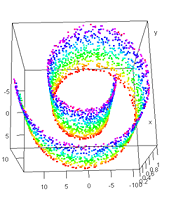
\includegraphics[width=\textwidth]{swisroll.png}
   \\swiss-roll
   \end{minipage}\hfill
   \begin{minipage}[c]{0.45\linewidth}   
      \centering 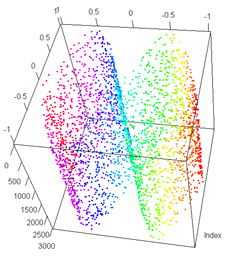
\includegraphics[width=\textwidth]{twinpearks.png}
   \\twinpeaks
   \end{minipage}
   \begin{minipage}[c]{0.45\linewidth}
      \centering 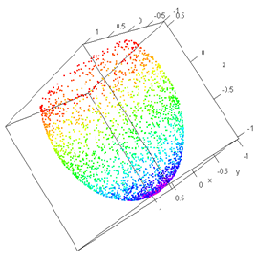
\includegraphics[width=\textwidth]{fishbowl.png}
   \\fishbowl
   \end{minipage}\hfill
   \begin{minipage}[c]{0.45\linewidth}   
      \centering 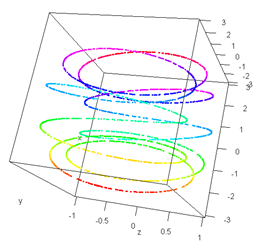
\includegraphics[width=\textwidth]{helix.png}
   \\Helix
   \end{minipage}
   \caption{graphique des données artificielles en 3D}
   \label{data_art}
\end{figure}


\subsection{Données réelle: Wine recognition}
 
Ces données proviennent de plusieurs industries italiennes d’analyse chimique, ils analysent les vins produits par $3$ viticulteurs. Selon les analystes le vin contient $13$ différents facteurs (quelques facteurs: Alcohol, Malic acid, Ash, Alcalinity of ash, Magnesium, Total phenols). Ce data set contient 14 variables dont 13 sont quantitatives et une qualitative qui représente les 3 groupes de producteurs. En outre elle ne contiens pas de valeurs manquantes ni de valeurs aberrantes. \href{http://archive.ics.uci.edu/ml/datasets/Wine
}{voir ce lien}

\section{Comparaison des méthodes}
L’efficacité, la puissance et la capacité des techniques de réduction à restituées la totalité de l’information peuvent être comparés sur plusieurs aspects : locaux et globaux. Il existe cependant plusieurs  critères relatifs à la mesure de la qualité de l’information: le Critère de la continuité locale, de fiabilité, de Mean Relative Rang Error, de Rang d’Erreur Moyenne Relative, d’Entropie, de la variance et de la dérivée Spectral d’Ordre $1$. Nous  allons utiliser le critère de fiabilité pour évaluer nos différentes techniques. \cite{Maaten08}

\subsection{ Comparaison numérique}
La continuité MC est une mesure de la bonté des techniques de réduction, elle considère le fait que les positions dans l’espace réduit (dimension $d$) doivent être égales à celle de l’espace initial, en plus elle calcul le degré de la continuité des différents points qui sont dans le voisinage. Soit  $V_{k}(y_i)$ l’ensemble des points qui ont été projetés, mais qui ne se trouve pas dans de voisinage $y_i$. Par contre ses points coïncident dans l'espace d’origine dont le voisinage est $x_i$. La valeur de MC est définie entre $0$ et $1$ \cite{Khoder13}
\[ \mathbf{S}= 1-A(k)  \sum_{i=1}^{n}\sum_{y \in V_{k}(y_i)}^{} (\hat r(y{_i}, y{_j} -k)\] sachant que: $\mathbf {A_K}= 1- \frac{2}{nk} (2n-3k-1)$ \\ et $\mathbf {V_{k}(y_i)}=  \{ {y_j} /\quad {y_j} \not\in 
\hat C{_k}(Y_i) \cap \in C{_k}(y_i)\}$ \cite{Wang12} \cite{Maaten08}



\subsection{Comparaison empirique et théorique}

Pour une étude de comparaison, nous devons aussi évaluer d’autres aspects : optimisations et de décompositions spectrales réalisées, algorithmique.
L’ACP comme la MDS fonctionne très bien quand on a des données linéaires, ils sont souvent équivalents s’ils contiennent les mêmes auto-valeurs de la matrice de corrélation. Par contre La MDS se base sur la matrice de Gram de produits scalaires. 
Ils ont des limites pour les données complexes.  Ils sont limités par  leur contrainte de linéarités.
L’Isomap et LLE sont des exemplaires du Kernel PCA, elles sont aussi basées sur  matrice de Gram. Cette matrice est obtenue en utilisant la  théorie des graphes (relations de voisinages) pondérés contrairement à une fonction prédéfinie, les noyaux obtenus sont considérés « indépendante ».Ses deux technique sont complexes et sensibles aux  différentes variations (paramètres) des lors que nous avons des données de grande dimension à cause de la complexité de leurs algorithmes. Par contre la LLE s’avère souvent plus plus puissante et efficiente que l’ACP, la MDS et l’ISOMAP

\subsection{Complexité,  mémoire et paramètre}
La table ci-dessous nous donnes un résumer sur les paramètres utiliser afin d’avoir la technique optimale. Soit $n$ est la taille de la matrice $k$ le voisinage $p$ la proportion d’élément non nul contenu dans la matrice creuse par rapport au nombre total d’éléments. $w$ est poids du réseau après chaque itération \cite{Maaten08} \\

\begin{tabular}{|l|c|r|l|c|}
  \hline
  Technique & paramètre   & complexité & mèmoire\\
  \hline
  PCA & No & $O(n^3)$ & $O(n^2)$\\
  MDS & No  & $O(n^3)$ & $O(n^2)$\\
  ISOMAP & $ 5 \le k \le 15 $ & $O(n^3)$ & $O(n^2)$\\
  LLE & $5 \le k \le 15$  &  $O(pn^2)$ & $O(pn^2)$\\
  Sammon& No  & $O(n^3)$ & $O(n^2)$ \\
  \hline
\end{tabular}
\\
%------------------------------------------------
\section{Résultat des expériences et discutions}
Nous avons essayé les différents techniques sur des données simulées et réelle. 
Pour le  cas des données artificielles nous avons introduit des bruits afin de faire une étude comparative et de chercher à comprendre le comportement de certaines méthodes face aux données bruités, ensuite nous avons mesuré le temps pour chaque cas d’études, ceux-ci permettant de calculer la vitesse d’exécution des algorithmes. Cependant  ce critère n’est pas optimal car il dépend de plusieurs paramètres (processeur des ordinateurs, paramètre k, dimension des données et du bruit), c’est pour cette raison que nous avons utilisé le critère  de trustworthinees ou fiabilité  qui est plus cohérent.\\

Pca et Sammon sont deux méthodes non paramétrique mais sammon a implicitement un paramètre de réglage k qui représente la dimension réelle du jeu de donnée. Nous avons choisi $k=2$ car nous connaissons que la vrai dimension est égale à $2$.\\
LLE et isomap sont paramétrique la première a deux paramètre ($k$ et $m$), $k$  donne le nombre optimal de voisin. Son algorithme nous a donné un résultat optimal de $k=15$ (voir figure \ref{kopt_lle}) pour nos jeux de données. Le second paramètre $m$ équivaut à la dimension réelle. Pour isomap le paramètre $k$ correspond au voisin le plus proche, elle n’est pas robuste si la distribution des données n’est pas uniforme et la sélection du $k$ optimal n’est pas facile vue que la distance mesurée ne peut pas être trouvé facilement quand la distance géodésique est plus courte .

\begin{figure}[ht!]
 \centering
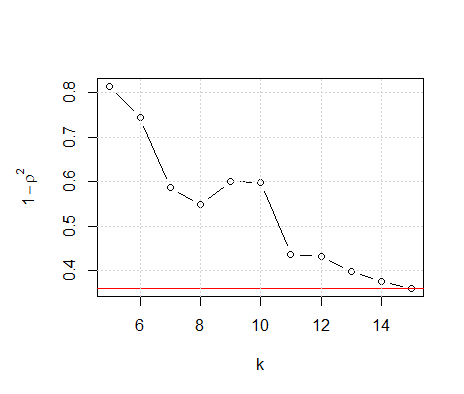
\includegraphics[width=\linewidth]{ff.png}
\vspace{-20pt}
 \caption{LLE: graphique pour k optimal}
 \label{kopt_lle}
\end{figure}

Pour notre étude nous  avons étudié $4$ cas possibles pour le paramètre $k$ afin de voir son effet sur les données
Cas 1: 
LLE: $k=15$ valeur optimal pour le LLE évaluer par représentation graphique et numérique, voir figure 
Isomap: $k=15$ valeur optimal pour le Isomap  \\
Cas 2: 
LLE: $k=8$,   Isomap: $k=6$\\
Cas 3: 
LLE: $k=13$, Isomap: $k=8$\\
Cas 4:
LLE: $k=3$,   Isomap: $k=3$

Visuellement, nous pouvons détecter la meilleure réduction en éliminant toutes représentations des points de différents couleurs entremêlés, ce qui indique une erreur dans la reconstruction de la complexité de la structure. On remarque que les méthodes choisi dans chaque simulation ont réussi à reconstruire la structure non linéaire du jeu de données original, en dépliant les dimensions et les reproduisant en deux dimensions.

Pour le jeu de donnée  Swiss-Roll (figure \ref{swiss}  la méthode LLE est la plus satisfaisante pour la réduction de dimension car la valeur de fiabilité est plus grande que les autres, par contre elle a un temps de calcul trop long. (figure\ref{res})

\begin{figure}[ht!]
 \centering
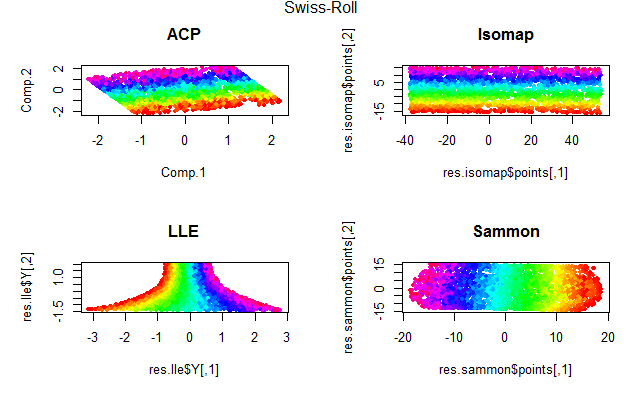
\includegraphics[width=\linewidth]{sreduit.png}
\vspace{-20pt}
 \caption{Swiss roll réduit en 2D}
 \label{swiss}
\end{figure}

Pour les données FishBowl (figure \ref{fish}) la méthode  PCA est la plus approprie avec la plus forte valeur calculée pour le critère de fiabilité ou “Trustworthiness” en plus elle a un temps de réponse relativement cour. (Voir figure \ref{res})

\begin{figure}[ht!]
 \centering
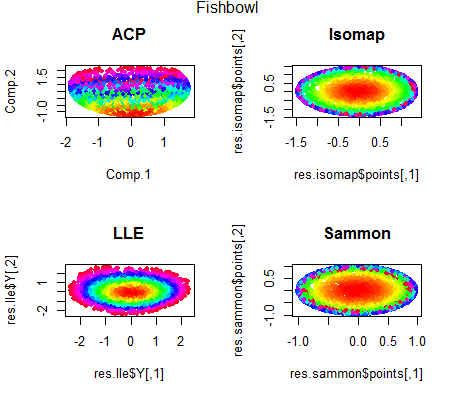
\includegraphics[width=\linewidth]{f.png}
\vspace{-20pt}
 \caption{Fishbowl en 2D}
 \label{fish}
\end{figure} 

Pour le jeu de donnée Helix (figure \ref{helix}) la méthode Sammon réussi a garder la forme des données et a un critère de fiabilité égal à $1$. (voir figure \ref{res})

\begin{figure}[ht!]
 \centering
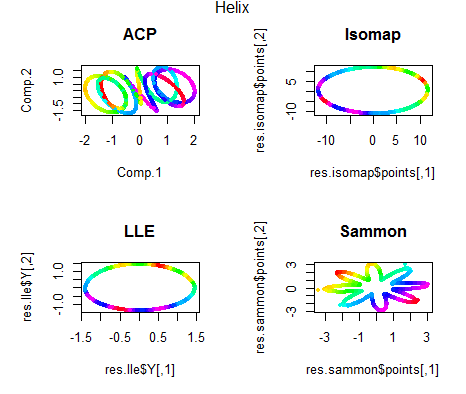
\includegraphics[width=\linewidth]{hh1.png}
\vspace{-20pt}
 \caption{helix réduit en 2D}
 \label{helix}
\end{figure} 
Pour les données réelles la méthode sammons semble être la meilleur (voir figure \ref{res}) mais vue la structure des données (les 3 classes sont linéairement séparables) on pouvait s’attendre à voir l’acp comme la méthode adéquate pour ce data set (voir figure \ref{wine}).

\begin{figure}[ht!]
  \centering
  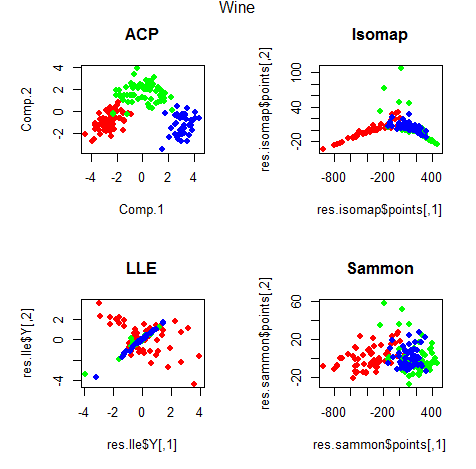
\includegraphics[width=\linewidth]{wine.png} 
  \vspace{-10pt}
  \caption{wine dimensionality}
  \label{wine}
\end{figure}

\begin{figure*}[!htbp]
  \centering
  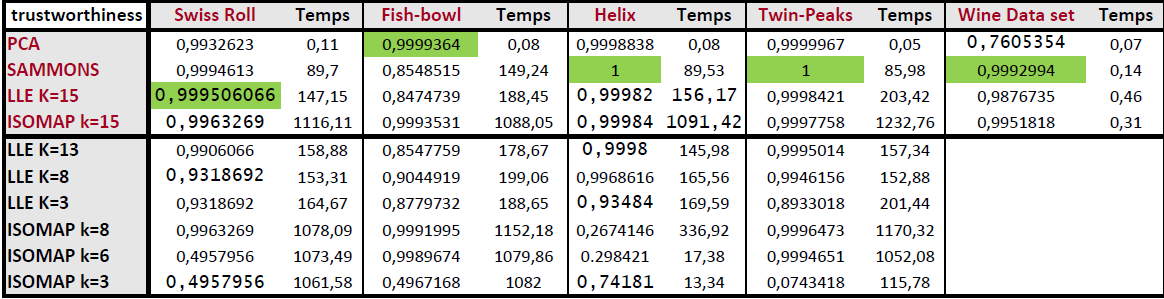
\includegraphics[width= \linewidth]{resul.png} 
  \vspace{-10pt}
  \caption{tableaux résultat}
  \label{res}
\end{figure*}

Pour temps des calculs, on observe en ordre décroissant: Isomap, LLE, Sammons et PCA (Figure \ref{res}).\\
L'analyse comparative prise des données avec et sans bruit indique une méthode différente pour chaque jeu de données. L’ajout du bruit augment le temps d’exécution des algorithmes et rend certaines techniques vulnérables.

\section{Conclusion }
Ils existent plusieurs méthodes pour la réduction de la dimension. Dans cette étude comparative ils émergent plusieurs résultats intéressants,les techniques dépendent de quelques paramètres :
\begin{itemize}
\item Natures, dimension et formes des données
\item Niveau de bruit introduit
\item Type de distance choisi  
\item Valeur optimal du paramètre k
\end{itemize}A la lumière de cette études nous pouvons conclure que aucun de ses techniques n’est parfaites, chacune d’entre elles présentent des avantages et inconvenant.
Certaines méthodes convergent très vite mais sont par contre sensible aux bruits, d’autres ont d’excellent résultats quand les données sont linéaire. Enfin d'autres ne souffrent pas de l'effet "grande dimension". Malgré la capacité des techniques non linéaires à réduire la dimension des données réelles il résulte que la pca est très souvent adapté pour la réduction de la dimension. Nous n'avons pas explorer d'autres techniques comme la kernel pca, Autoencoder, Laplacian
Eigenmaps, Diffusion maps et LTSA.\\

Dans le futur nous devons nous concentrer sur le développement des techniques non linéaires qui ont un temps computationnel acceptable, qui prennent en compte le cas des données manquantes ou aberrantes et qui ne souffre pas des solutions non convexe.

%----------------------------------------------------------------------------------------
%	REFERENCE LIST
%----------------------------------------------------------------------------------------
  \bibliographystyle{plain}
\bibliography{bibliographie.bib}

%----------------------------------------------------------------------------------------

\end{document}
